\documentclass{article}


\usepackage{arxiv}

\usepackage[utf8]{inputenc} % allow utf-8 input
\usepackage[T1]{fontenc}    % use 8-bit T1 fonts
\usepackage{hyperref}       % hyperlinks
\usepackage{url}            % simple URL typesetting
\usepackage{booktabs}       % professional-quality tables
\usepackage{amsfonts}       % blackboard math symbols
\usepackage{nicefrac}       % compact symbols for 1/2, etc.
\usepackage{microtype}      % microtypography
\usepackage{multicol} 
\usepackage{lipsum}
\usepackage{graphicx}
\usepackage{sidecap}

\sidecaptionvpos{figure}{c}

%\title{Glyph embeddings for machine translation \emph{arxiv}}
\title{Glyph embeddings for machine translation}

\author{
  Bailey Polonsky\thanks{This project was completed in cooperation with Kuan Yu of Potsdam University \emph{kaunyu@uni-potsdam.de}.} \\
  Neural Machine Translation Course\\
  Potsdam University\\
  14469 Potsdam \\
  \texttt{baileypolo@gmail.com} \\
  %% examples of more authors
  %% \AND
  %% Coauthor \\
  %% Affiliation \\
  %% Address \\
  %% \texttt{email} \\
  %% \And
  %% Coauthor \\
  %% Affiliation \\
  %% Address \\
  %% \texttt{email} \\
  %% \And
  %% Coauthor \\
  %% Affiliation \\
  %% Address \\
  %% \texttt{email} \\
}

\begin{document}
\maketitle
\begin{abstract}
Modern neural networks used for language modeling rely on word- or character-level embeddings to represent the semantic relationship between components. This paper proposes a new approach: glyph-level embeddings for rendering a semantic space from the glyph images of the text's font. This approach offers exciting new possibilities for translating logographic languages based on sub-character meanings or translation of entire sentence level glyphs without auto-regressive token dependency. We develop a baseline test for glyph embeddings, comparing the efficacy of various different embedding and inference modes using Latin languages as a controlled sample, and a small recurrent auto-regressive model for translation. Our experiments demonstrate that even without glyph-level significance in an language (ie, non-logographic languages), glyphs can be used as an effective medium for both semantic embedding \emph{and} inference production, paving the way for possible improvements on existing translation methods. 
\end{abstract}

\section{Introduction}
Natural language processing is a field dedicated to negotiating the significant translations between organic human language and the minimalist representations of information in a computer system. Computers generally operate on language represented by a writing system, internally described to the computer with unique byte codes, each representing a character symbol. For example, the common character encoding scheme UTF-8 uses between eight and thirty-two bits to map to over a million distinct characters. Linguistic processing techniques often treat these discrete units as a sequence of base-level items which can be fitted together to represent higher-level language components. This is in contrast to the human visual system, which interacts with written text in a process of skips and fixations, rather than a sequence of discrete characters which add up to an orderly composite \cite{eyefixation}.

Language processing efforts have been hampered by the inability of models to reliably connect related components of a text sequence over irregular distances in organic language. Trends away from linear interpretations of text sequences have proved to be effective in the task of language modeling, with attention mechanisms in particular providing a suggestive new direction for language modeling \cite{attnisalluneed}.

Projecting semantic information into a learned vector space provides a number of advantages: improving training by sharing semantic context with models, reducing data load in lower dimensions than one-hot vectors, the possibility of incorporating semantic information from larger vocabularies already trained on the embedding, etc. Neither are embeddings are limited to word-level semantics, the well known skip-gram and CBOW models are developed to incorporate phrase or sentence level contexts into the semantic representation space. Likewise, finer granularity can be effective, character level embeddings have been shown to results when used concurrently with word level embeddings \cite{yinmultigran2016}.

It is not intuitive that there might be a useful embedding level below the character component. The Latin alphabet, for example, is composed of a low number of characters, and many phonemes are represented by more than a single character. In this context, one could easily assume that there is no useful information that a learned embedding could extract from the shape of a single character as opposed to the character as a discrete class.

This intuition does not hold with all languages. Non-alphabetic writing systems, such as used in Chinese or Japanese, often use characters comprised of semantically rich radicals. However, because radicals are generally discrete symbolic structures, combined to form larger characters, research on radical embedding tends to treat them as specific values which are rearranged to form characters, rather than continuous shapes to be read in context \cite{yinmultigran2016, jpcn2017glyph} 

Our project expands on that research, comparing glyph-level embeddings and inference in the translation of alphabetic writing systems. By controlling for semantic significance, we demonstrate in this paper that glyph-level representations of language can be useful for a variety of purposes in computer modeling of language. Our experiments establish baseline comparisons between models trained to regenerate both glyph and string translations of a glyph encoder, as well as comparing the efficacy of glyphs as tools for inference and tools for training. 

We use the Europarl paired corpus to translate German source text to English \cite{euro}. Our glyphs are generated from Google NOTO monospace font. We implement a commonly used recurrent autoencoder system for translation, including as adding a simple attention layer to accommodate longer sequences and attenuate some of the sequence length decay associated with RNNs. Although recurrence is not strictly necessary for glyph to glyph encodings, as will be shown, this architecture allows for fair comparison between various types of training and inference inputs. 


\section{Related Work}


\label{sec:related works}

 Related work is broken into two parts, a description of the existing research on glyph embeddings in logographic languages and a brief background on the architectures used in this paper.

\subsection{Embedding Logographic Writing}
\label{sec:Logographic radicals}
Logographic writing systems are the the clearest possibility for glyph embedding to improve a model's semantic comprehension. Normally the radicals in those languages that could carry this semantic information are generally treated as discrete sub-characters. Radical embedding has been shown to be particularly effective in logographic-to-logographic translations \cite{jpcn2017glyph}. As lower-level components of written text, radicals have been incorporated as the entire language representation, or as multi-granularity models which generate embeddings for radicals and string-characters, and then feed both of those embeddings forward into a language model \cite{shi2015, yinmultigran2016}. 

Some research carries this multi-granularity modeling further towards a glyph model of whole radical-composed characters (ie, a glyph not of individual radicals but of their composition in characters.) Su and Lee found that while glyphs of entire characters could model language effectively on their own, but could be used in a multi-granular model to improve semantic clustering, as well as to improve CBOW and Skipgram language modeling \cite{su2017}. This essential concept of autoencoding the images of the glyph set is the core technique of our baseline modeling.

\subsection{Model Architecture}
\label{sec:Model architecture}
We implemented a variation of the well-developed bidirectional RNN encoder-decoder structure as a baseline for glyph embedding tests \cite{bidirectionalrnn}. In fact, the model is an autoregressive network, conditioned not on a hidden state but on the outcome of previous steps in the network \cite{autoregression}. A single attention layer with eight heads and residual connections was added after the decoder. 

This model is commonly used because it has several advantages for language work on a string level. The bidirectional series can carry information from everywhere in the source sentence for translation and the sequence-conditioned inference is intuitive to the sequence-conception of a string of bits.  On the other hand, the model is particularly badly suited to a glyph level input. It restricts inputs to discrete time points--unnecessary if the model can "read" directly from a whole sentence of glyphs \ref{sec:Future Works}. The autoregression is also an unhelpful limitation for glyph-representations. Even glyphs parted into single characters are entirely determined on inference--any confusion is represented in a "fuzzy" glyph output, rather than some probability distribution that needs sampling.

We conducted experiments with an autoregressive RNN, and without logographic components in the translated languages in order to isolate glyph embedding as cleanly as possible in comparison to a string embedding. Our model architecture and data have been developed to accommodate linear strings of input: the parity our glyph embeddings achieve are therefore a demonstration of their core usefulness. 

\section{Experimental Setup}

\subsection{Data}
From the Europarl paired corpus, we translated from German to English. Sentences with fewer than 3 or more than 256 characters were removed, and the least frequent characters representing less than 00.05\% of tokens were UNKed (99.95\% coverage). The latter was solely for the benefit of the character models, as glyphs can represent any character regardless of its frequency.

Glyphs were generated from Google's NOTO sans mono font, a font format which ensures that each glyph in a particular language fits to the same size bitmap. 

\subsection{Experimental Modes}

Both the format of the data input during training, and the output's of the model used for evaluation and inference were varied in the experiment.

\subsubsection{Model Inputs}
Rather than simply produce models which converted glyph inputs to glyph outputs, we varied the character representation strategy at several points in the model. The source inputs to the encoder, the encoder output to the decoder, and the character representation at the output were all varied between strings and glyphs. In the case of source input, the character embedding was changed, in the case of the decoder input the context input to the decoder is embedded as a glyph, and in the case of output, the loss function was calculated against either the output of the model as a glyph or a string. These formats are referred to in their order in the model, eg. string characters at each step are ccc, a string character embedding to the encoder followed by glyph decoding and inference is cgg, etc.

Not every format variation was tested during experiment. ccc, ggg, ccg, and cgg were tested. 

It is important to note that in every variation of the model, both a character string and a glyph were output by the graph, useful for varying inference modes. In xxg models, the model was trained on the loss of the glyph output with a 1/10th-factor contribution from the character output, and in xxc models the model was trained only on the loss of the character output.

\subsubsection{Inference Modes}
Five modes were used for inference, as seen in Table \ref{tab:table1}. Inference feedback was varied between the glyph output from the model, output glyphs "corrected" to match the closest glyph bitmap (calculated by subtracting output glyphs from all font-rendered glyphs in the language), glyphs rendered from the highest probability character output, and a rendering of each glyph weighted by its probability in the character output. 

The BLEU scores needed to be converted back to strings, and inference modes vary between using the \verb+argmax(character string distribution)+ and the character whose glyph was the least distant from the model's output character.

Because some inference modes required a glyph output, not every input format was tested with every mode.

\begin{SCfigure}
\centering
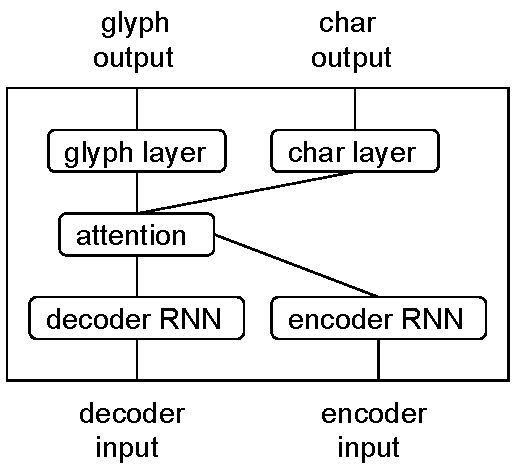
\includegraphics[width=0.35\linewidth]{architecture.pdf}
\caption[]{\label{fig:arch} Model architecture. Model format is indicated by x,y,z notation where x the format input to encoder, y is input to decoder and z is the trained output, character or glyph. Diagram courtesy Kuan Yu.}
\end{SCfigure}

\begin{table}
  \centering
  \caption{Inference Modes.}
  \begin{tabular}{lccc}
    \toprule
    \cmidrule(r){1-2}
    Mode  & Inference Feedback & BLEU Score & Applicable Formats\\ 
    \midrule
    1     & Glyph  & argmax(string)   & cgg, ggg  \\
    2     & Glyph & Glyph matched to nearest char & cgg, ggg    \\
    3     & Rendered corrected glyph & Glyph matched to nearest char & cgg, ggg  \\
    4     & Rendered argmax(string distribution) & argmax(string) & all\\
    5     & Rendered probs over string distribution & argmax(string) & all\\
    \bottomrule
  \end{tabular}
  \label{tab:table1}
\end{table}

\section{Results}

BLEU scores were calculated for the respective inference modes used, using SacreBLEU \cite{bleu}. The results can be seen in Table 2. It should be noted that ccc training quickly overfitted when introduced to the same hyperparamaters, whereas the other formats were trained on the data for 60 epochs, ccc's training was terminated after 30 epochs due to speedy overfitting.

As can be seen in the results, the best BLEU scores are achieved by character-based formats, using glyphs rendered from characters. Regardless of training format, the BLEU scores for inference mode 4 closely match, suggesting that the models make relatively little differentiation between input formats, but perform best with discrete character inference. The higher performace of glyph-first models in mode 5 over mode 1 further suggests that inference is improved by using context from the string characters.

However, there are significant details that suggest some value encoded by the glyphs that cannot be encoded by characters. In mode 5, models trained on glyphs outperformed models trained in characters. That is to say, when the probability distribution is represented as a glyph, glyph-based models can learn more from the context than can characters based models.

The largest failing of the glyph models is in inference from their own output. In all cases, cleaned glyphs, or glyphs generated from character probability distributions outperform the gylph models inferring on their own. 

\section{Discussion}

These results are initially discouraging, but demonstrate several useful properties of glyph embedding models. Firstly, the models are capable of near-parity with string-based embeddings when both are trained as outputs. This is in contrast to the multi-granularity techniques discussed in Section 2.1, which used both embeddings together as input during training. It could be the case that character outputs act as a regularizer to improve the learning in a glyph-embedded model. 

It is also notable that models could perform at parity when doing inference from glyphs of any kind. Inference via glyphs shortcuts typical probabilistic searches when selecting the next element to add to the sequence. As can be seen in Section 5.2.1 the ambiguity that confuses string-based inference is nevertheless legible to both humans and glyph-inference readers. Glyphs also prove useful for UNKed characters, without particular input 
can decipher what an UNKed string cannot.

\subsection{Future Work}
\label{sec:Future Works}

There are a number of promising directions to improve on. The connections between embeddings and RNN layers were simple dense linear transformations. It makes much more sense to use a convolutional layer to help train the model, particularly in the case of fuzzy inferences which may have confused parts of the character representation. Convolutions have, in any case, been shown to be useful in radical-based embeddings as radicals can be translated or transformed from one character to another character. 

Another exiting potential route is the possibility of doing away with character sequencing altogether, and simply translating whole sentence-glyphs into a target language. Attention networks and even GANs have been shown to perform well at image-to-image translation \cite{imagetrans}.

\begin{table}
  \centering
  \caption{Results}
  \begin{tabular}{lccccc}
    \toprule
    \cmidrule(r){1-2}
    Format  & Mode 1 & Mode 2 & Mode 3 & Mode 4 & Mode 5\\ 
    \midrule
    ccc     & -  & - & - & {\bf 30.9} & 20.3 \\
    cgc     & - & - & - & {\bf 30.9} & 22.4  \\
    cgg     & 22.9 & 23.5 & 26.5 & {\bf 30.9} & {\bf 24.1} \\
    ggg     & 21.9 & 22.2 & 25.3 & 30.2 & 23.0 \\
    \bottomrule
  \end{tabular}
  \label{tab:table2}
\end{table}

\subsection{Example texts}
\subsubsection{Ambiguous Inference}
The format in this example is source glyph, target glyph, cgg glyph inference, ggg glyph inference, cgg string inference and ggg string inference.

\vspace{1.2em}\noindent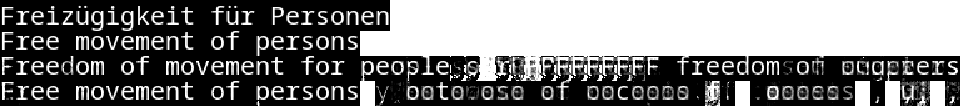
\includegraphics[width=\linewidth]{038.pdf}
\texttt{cgg}: \texttt{Free om of movement for people███████████████free om on migpeers}\\
\texttt{ggg}: \texttt{Free movement of persons█y brto ovc of tucomaa o.█.ortei █.██(█(}\\
\vspace{-0.8em}

\subsubsection{UNK recognition}
The format in this example is source glyph, target glyph, cgg glyph inference, ggg glyph inference, cgg string inference and ggg string inference.

\vspace{1.2em}\noindent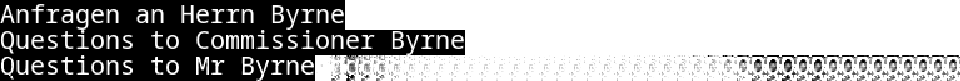
\includegraphics[width=\linewidth]{019.pdf}
\texttt{cgg}: \texttt{?uestions to Cr Byrne███████████████████████████████████████████}\\
\bibliographystyle{unsrt}  


%\bibliography{references}  %%% Remove comment to use the external .bib file (using bibtex).
%%% and comment out the ``thebibliography'' section.


%%% Comment out this section when you \bibliography{references} is enabled.
\begin{thebibliography}{1}

\bibitem{eyefixation}
Just, Marcel Adam, and Patricia A. Carpenter. 
\newblock"Eye fixations and cognitive processes." Cognitive psychology 8.4 (1976): 441-480.

\bibitem{attnisalluneed}
Vaswani, Ashish, et al. 
\newblock"Attention is all you need." Advances in Neural Information Processing Systems. 2017.

\bibitem{yinmultigran2016}
Yin, Rongchao, et al.
\newblock "Multi-granularity chinese word embedding." Proceedings of the 2016 Conference on Empirical Methods in Natural Language Processing. 2016.

\bibitem{su2017}
Su, Tzu-Ray, and Hung-Yi Lee
\newblock "Learning chinese word representations from glyphs of characters." arXiv preprint arXiv:1708.04755 (2017).

\bibitem{jpcn2017glyph}
Ke, Yuanzhi, and Masafumi Hagiwara. 
\newblock"Radical-level Ideograph Encoder for RNN-based Sentiment Analysis of Chinese and Japanese." arXiv preprint arXiv:1708.03312 (2017).

\bibitem{euro}
Koehn, Philipp. 
\newblock "Europarl: A parallel corpus for statistical machine translation." MT summit. Vol. 5. 2005.  Jacovi.

\bibitem{bidirectionalrnn}
Schuster, Mike, and Kuldip K. Paliwal. 
\newblock "Bidirectional recurrent neural networks." IEEE Transactions on Signal Processing 45.11 (1997): 2673-2681.

\bibitem{autoregression}
Gregor, Karol, et al. 
\newblock "Deep autoregressive networks." arXiv preprint arXiv:1310.8499 (2013).

\bibitem{gru}
Chung, Junyoung, et al. 
\newblock"Empirical evaluation of gated recurrent neural networks on sequence modeling." arXiv preprint arXiv:1412.3555 (2014).

\bibitem{shi2015}
Shi, Xinlei, et al. 
\newblock"Radical embedding: Delving deeper to chinese radicals." Proceedings of the 53rd Annual Meeting of the Association for Computational Linguistics and the 7th International Joint Conference on Natural Language Processing (Volume 2: Short Papers). Vol. 2. 2015.

\bibitem{bleu}
Post, Matt. 
\newblock"A call for clarity in reporting bleu scores." arXiv preprint arXiv:1804.08771 (2018).

\bibitem{imagetrans}
Isola, Phillip, et al. 
\newblock "Image-to-image translation with conditional adversarial networks." Proceedings of the IEEE conference on computer vision and pattern recognition. 2017.

\end{thebibliography}


\end{document}
